%-----------------------------
\section{MST und Kruskal}
\subsection{MST}

\begin{frame}
\frametitle{Minimum Spanning Tree (MST)}
\begin{itemize}
\item "finde das billigste Netzwerk"
\item genau: \\
Gegeben sei ein zusammenhängender ungerichteter gewichteter Graph, gesucht ist ein zusammenhgängender Teilgraph mit geringstem Gesamtgewicht.
\end{itemize}
\end{frame}

\begin{frame}
\frametitle{Lösung}
\begin{itemize}
\item Ansatz: baue einen Baum mit greedy Algorithmus:
\begin{enumerate}
\item betrachte Kante mit niedrigstem Gewicht
\item untersuche: führt hinzufügen der Kante zu einem Zyklus?
\begin{itemize}
\item Ja: verwerfe Kante
\item Nein: füge Kante zum Baum hinzu
\end{itemize}
\item starte bei 1. mit restlichen Kanten bis alle abgearbeitet sind
\item $ \implies $ Baum ist ein MST
\end{enumerate}
\end{itemize}
\end{frame}

\begin{frame}
\frametitle{Lösung}
\begin{figure}
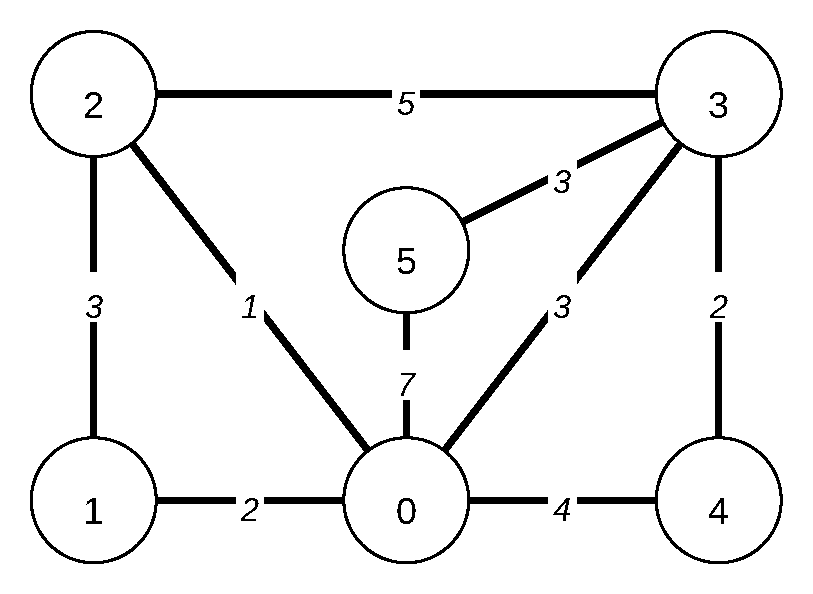
\includegraphics[width=0.75\linewidth]{kruskal_graphs/graph1.pdf}
\end{figure}
\end{frame}
